\documentclass[12pt]{article}

\usepackage{sbc-template}
\usepackage{graphicx,url}
\usepackage[utf8]{inputenc}
\usepackage[brazil]{babel}

\sloppy

\title{(?)\footnote{Omitido para revisão.} : UM AMBIENTE DE TECNOLOGIAS DE APOIO PARA O ENSINO DE LÓGICA DE PROGRAMAÇÃO}

\author{$\textbf{(?)}$ \inst{1}, $\textbf{(?)}$ \inst{1}, $\textbf{(?)}$ \inst{1}, $\textbf{(?)}$ \inst{1}}

\address{$(?)$
  \email{\{$(?)$, $(?)$,  $(?)$, $(?)$\}@gmail.com}
}

\begin{document} 

\maketitle

\begin{abstract}
This article is an improvement on a previous work. It is a tool to aid in the learning process of students in programming logic content. We implement graphic resources on logical structures which facilitate the learning process of the concepts inherent to the initial discipline of the Technical Course in Computer Science. The application is being developed on the web platform and will consist of visual programming based on programming blocks, flowcharts and application of the cognitive domain of the Revised Bloom Taxonomy. It is intended to use gamification resources in order to stimulate students in the study of the discipline and in the best assimilation of the concepts of logic. The prototype was applied to students of the first year of high school, in order to collect information on ease of use and identification of the block structures used in the program. Preliminary results show that the software meets the proposal simply and easily.
\end{abstract}
     
\begin{resumo}
Este artigo é uma melhoria de um trabalho anterior. Trata-se de uma ferramenta para auxiliar no processo de aprendizagem de estudantes na disciplina de lógica de programação. Para facilitar, utilizou-se representações de recursos gráficos baseados em estruturas lógicas que facilitam o aprendizado dos conceitos inerentes à disciplina inicial do Curso Técnico Integrado em Informática. A aplicação está sendo desenvolvida na plataforma web e consistirá na programação visual com base em blocos de programação, fluxogramas e na aplicação do domínio cognitivo da Taxonomia de Bloom Revisada. Pretende-se utilizar recursos de gamificação a fim de estimular os alunos no estudo da disciplina e na melhor assimilação dos conceitos da lógica. O protótipo foi aplicado para alunos do primeiro ano do ensino médio, com o objetivo de recolher informações sobre facilidade de uso e identificação das estruturas de bloco utilizadas no programa. Os resultados preliminares mostram que o software atende a proposta com simplicidade e facilidade.
\end{resumo}

\section{Introdução} 
Algumas dificuldades inviabilizam a compreensão da programação desde a abordagem utilizada para o ensino até o aspecto cognitivo do aluno. Segundo \cite{GOMES:2008}, dentre os possíveis fatores deste problema destacam-se o elevado nível de abstração da programação e a falta de motivação do próprio aluno. 
\par Em um estudo de caso baseado na Taxonomia de Bloom e no Scratch, realizado por \cite{ARAUJO:2013}, percebeu-se a necessidade de incentivo ao aprendizado e do uso de outros recursos visuais como base metodológica. Portanto, modificações na abordagem utilizada durante as aulas de lógica podem torná-las mais interativas e despertar gradativamente o interesse do aluno, apesar das possíveis dificuldades enfrentadas $(?)$.
\par O \textit{software} $(?)$ desenvolvido por $(?)$ dispõe de um ambiente de programação visual baseado em blocos e desenvolvido em Java Swing para ser empregado no aprendizado de lógica de programação, veja Figura~\ref{fig1}. Ele apresenta limitações, tais como: execução limitada a \textit{desktop} e conversão de algoritmo apenas para a linguagem C e para a utilizada pelo Arduino. Objetiva-se neste trabalho uma nova fase de desenvolvimento voltada para a plataforma \textit{web}, com conversão para multilinguagens e com a implementação de novas tecnologias que ampliem as funcionalidades para o público-alvo.
	\begin{figure}[h]
		\centering
		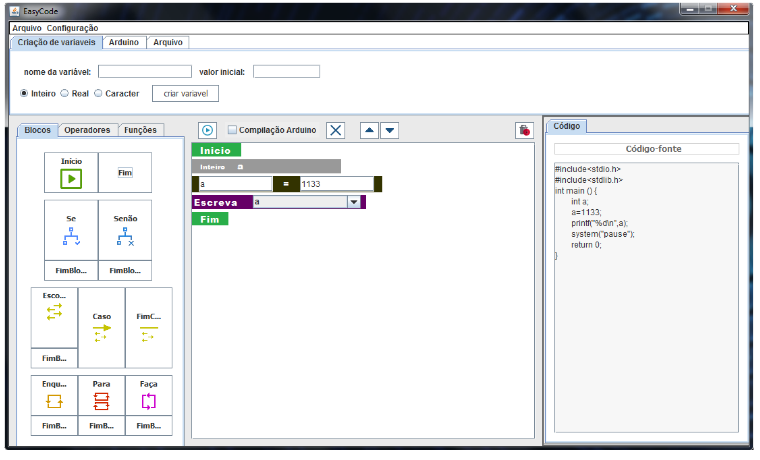
\includegraphics[scale=0.4]{2017.png}
		\caption{\textit{Layout} da tela principal do ambiente $\textbf{(?)}$.}
		\label{fig1}
	\end{figure}
	
\section{Metodologia} 
Utilizar-se-á o domínio cognitivo da Taxonomia de Bloom Revisada, que consiste nas categorias lembrar, entender, aplicar, analisar, avaliar e criar \cite{ANDERSON:2001} como atividades que o aluno deve realizar para que seja possível identificar o seu nível de aprendizado na disciplina de lógica. Esta será a base metodológica para a gamificação que será implementada na aplicação, que contará com uma sessão de desafios onde o discente poderá criar fluxogramas ou blocos (veja Figura~\ref{fig2}) e converter os códigos produzidos para as linguagens C, C++, Java, JavaScript e Python.
\par Ademais, a taxonomia em conjunto com pesquisas quanti-qualitativas serão aplicadas para alunos do primeiro ano do ensino médio técnico em informática do $(?)$ para avaliar o nível de desenvoltura na resolução de problemas computacionais a partir do \textit{software} $(?)$.
Além disso, os blocos visuais e a conversão entre multilinguagens de programação estão sendo implementados por meio da biblioteca Blockly da Google, permitindo que a ferramenta se torne mais atrativa para qualquer estudante.  

	\begin{figure}[h]
		\centering
		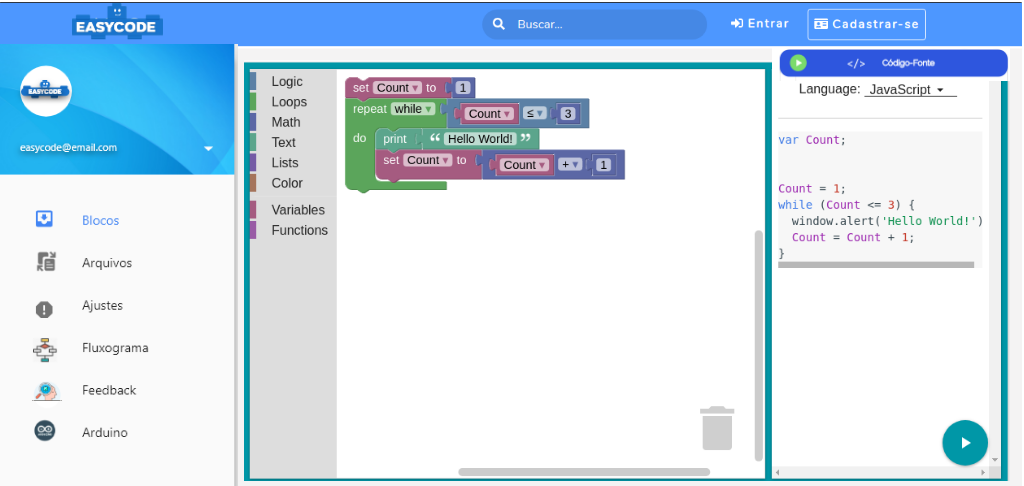
\includegraphics[scale=0.3]{bloc.png}
		\caption{Protótipo da tela de montagem de blocos do $\textbf{(?)}$.}
		\label{fig2}
	\end{figure}

\section{Resultados Parciais e Discussão}
No primeiro bimestre do ano de 2019, o protótipo apresentado na Figura~\ref{fig2} foi disponibilizado em um questionário e aplicado para cerca de 32 alunos do primeiro ano do Curso Técnico Integrado em Informática do $(?)$.
	\begin{figure}[!htbp]
		\centering
		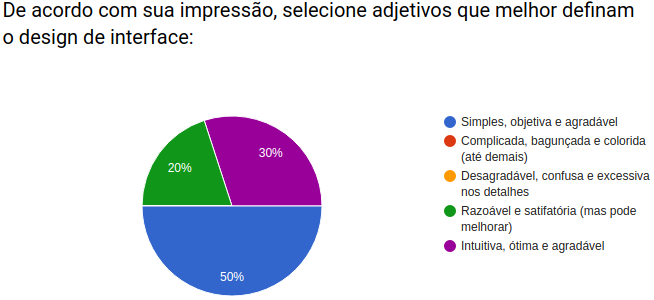
\includegraphics[scale=0.5]{g1.png}
		\caption{Gráfico relacionado ao \textit{design}.}
		\label{fig3}
	\end{figure}
\par Os resultados coletados e explicitados nos gráficos mostrados denotam que, no primeiro momento, os discentes avaliaram a \textit{interface} do \textit{software} (Veja Figura~\ref{fig3}) e a organização dos blocos de programação (Veja Figura~\ref{fig4}). Os alunos fizeram comentários positivos a respeito do protótipo, sugeriram a implementação de um \textit{chat} com a turma e apoiaram a ideia da gamificação com base em exercícios de lógica de programação.
	\begin{figure}[!htbp]
		\centering
		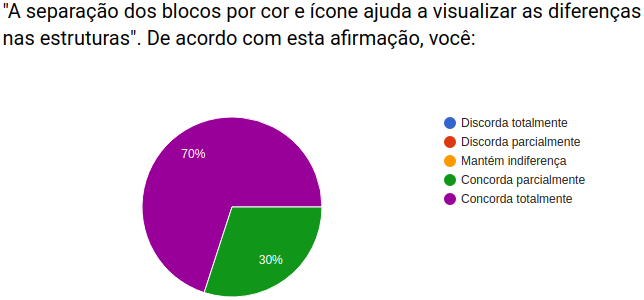
\includegraphics[scale=0.5]{g2.png}
		\caption{Gráfico em relação à organização dos blocos.}
		\label{fig4}
	\end{figure} 
\par As avaliações positivas dos alunos quanto ao protótipo demonstram que os mesmos estão aptos ao uso de novas metodologias de ensino dentro da sala de aula. Com esta expectativa, o \textit{software} proposto pode corroborar com o incentivo ao aprendizado de lógica de programação, pois a ferramenta visa atender os requisitos da nova geração de interação usuário-computador. 	

\section{Considerações Parciais}
O \textit{software} proposto é um ambiente que visa permitir que alunos com dificuldades de compreensão em lógica de programação possam aprender a programar de maneira mais prática. Espera-se que as mudanças propostas permitam que professores possam demonstrar de forma mais lúdica os conceitos da programação, por exemplo, possibilitando que os alunos compreendam as estruturas lógicas da disciplina.
\par Optou-se a utilização da plataforma \textit{web} devido à maior abrangência de uso do \textit{software}, pois sem a limitação \textit{desktop} haverá disponibilidade de acesso através de qualquer computador com acesso à \textit{internet}. Além disso, os blocos visuais e os processos dos fluxogramas servem como uma alternativa para instigar o aluno a associar a lógica ao código-fonte de várias linguagens de programação. 
\par Os próximos passos no andamento do trabalho são a implementação de recursos para a montagem de fluxogramas e, para permitir o engajamento do aluno e fomentar o uso da ferramenta, da gamificação baseada em competições, além da disponibilidade de criação de perfil para o acompanhamento do progresso do aluno. Também serão realizados testes com a ferramenta em sala de aula com o intuito de avaliar a desenvoltura do aluno na resolução de problemas lógicos por meio da aplicação de um questionário após as aulas práticas.

\bibliographystyle{sbc}
\bibliography{ArtigoEC}

\end{document}